\begin{figure}
	\begin{minipage}[b]{.55\linewidth}
		\centering
		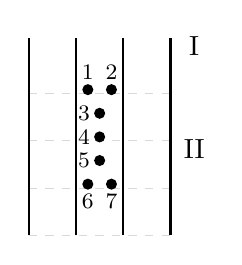
\begin{tikzpicture}		

		
			\GraphInit[vstyle=Normal]
			\tikzset{VertexStyle/.append style = {minimum size = 10pt, inner sep = 1.5pt}}
			
			\Vertex[x=2.4,y=2.1]{1}
			\Vertex[x=2.4,y=1.6]{2}
			\Vertex[x=3.4,y=2.1]{3}
			\Vertex[x=3.4,y=1.6]{4}
			\Edges(3,1,4,2)
			
			\Vertex[x=2.4,y=.8]{1}
			\Vertex[x=2.4,y=.3]{2}
			\Vertex[x=3.4,y=.8]{3}
			\Vertex[x=3.4,y=.3]{4}
			\Edges(1,3)
			\Edges(2,4)
			
			\node at (2.1,2.4){I};
			\node at (2.1,1.1){II};
				
			\draw[step=0.6,gray!30, dashed] (0,0) grid (1.8,2);
			\draw[thick] (0,0) -- (0,2.5);	
			\draw[thick] (.6,0) -- (.6,2.5);		
			\draw[thick] (1.2,0) -- (1.2,2.5);	
			\draw[thick] (1.8,0) -- (1.8,2.5);							
	
			\fill (.75,1.85) circle (2pt) node[anchor=south] {\footnotesize{1}};
			\fill (1.05,1.85) circle (2pt) node[anchor=south] {\footnotesize{2}};
			\fill (.9,1.55) circle (2pt) node[anchor=east] {\footnotesize{3}};
			\fill (.9,1.25) circle (2pt) node[anchor=east] {\footnotesize{4}};
			\fill (.9,.95) circle (2pt) node[anchor=east] {\footnotesize{5}};
			\fill (.75,.65) circle (2pt) node[anchor=north] {\footnotesize{6}};
			\fill (1.05,.65) circle (2pt) node[anchor=north] {\footnotesize{7}};
		\end{tikzpicture}
		\begin{tabular}{| c | c | c | c | c | c | c | c |}
			\hline
			$ id $     & 1 & 2 & 3 & 4 & 5 & 6 & 7 \\ \hline
			$ type $   & e & e & c & e & c & e & e \\ \hline
			$ cid_L $  & 1 & 1 & 1 & 1 & 2 & 2 & 2 \\ \hline
			$ cid_R $  & 3 & 3 & 3 & 4 & 4 & 4 & 4 \\ \hline
		\end{tabular}
		\subcaption{punkt brzegowy w różnych grupach}\label{qscan:qscan-problems-1}
	\end{minipage}%
	\begin{minipage}[b]{.45\linewidth}
		\centering
		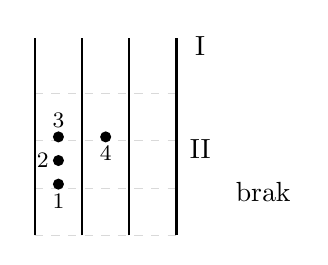
\begin{tikzpicture}		
		
		
		\GraphInit[vstyle=Normal]
		\tikzset{VertexStyle/.append style = {minimum size = 10pt, inner sep = 1.5pt}}
		
		\Vertex[x=2.4,y=1.85]{1}
		\Vertex[x=3.4,y=1.85]{2}
		\Edges(1,2)
		
		\node at(2.9, .55){brak};
		
		\node at (2.1,2.4){I};
		\node at (2.1,1.1){II};
		
		\draw[step=0.6,gray!30, dashed] (0,0) grid (1.8,2);
		\draw[thick] (0,0) -- (0,2.5);	
		\draw[thick] (.6,0) -- (.6,2.5);		
		\draw[thick] (1.2,0) -- (1.2,2.5);	
		\draw[thick] (1.8,0) -- (1.8,2.5);							
		
		\fill (.3,.65) circle (2pt) node[anchor=north] {\footnotesize{1}};
		\fill (.3,.95) circle (2pt) node[anchor=east] {\footnotesize{2}};
		\fill (.3,1.25) circle (2pt) node[anchor=south] {\footnotesize{3}};
		\fill (.9,1.25) circle (2pt) node[anchor=north] {\footnotesize{4}};
		\end{tikzpicture}
		\begin{tabular}{| c | c | c | c | c |}
			\hline
			$ id $     & 1 & 2 & 3 & 4 \\ \hline
			$ type $   & e & e & c & e \\ \hline
			$ cid_L $  & 1 & 1 & 1 & 1 \\ \hline
			$ cid_R $  & 2 & 2 & 2 & 2 \\ \hline
		\end{tabular}
		\subcaption{punkt brzegowy w MC}\label{qscan:qscan-problems-2}
	\end{minipage}
	\caption{Problemy pojawiające się przy scalaniu grup przy pomocy pola MC. Grafy zależności bez ignorowania (I) oraz z ignorowaniem (II) punktów brzegowych. $ e $ - punkt brzegowy, $ c $ - rdzeniowy}\label{qscan:qscan-problems}
\end{figure}